\subsection{Separating subset search from profiling}
\label{sec:ablation}
We use leave-one-out ablations and a cumulative ladder on 576 runs: sealed white noise (160), coloured noise (89), the hard 40, and three-dimensional \texttt{dysts} (287). No settings were tuned on these subsets. \Cref{fig:ladder} shows the ladder; full rates and paired tests are in \cref{tab:ablation,app:ablation-detail}.
\begin{figure}[t]
\centering
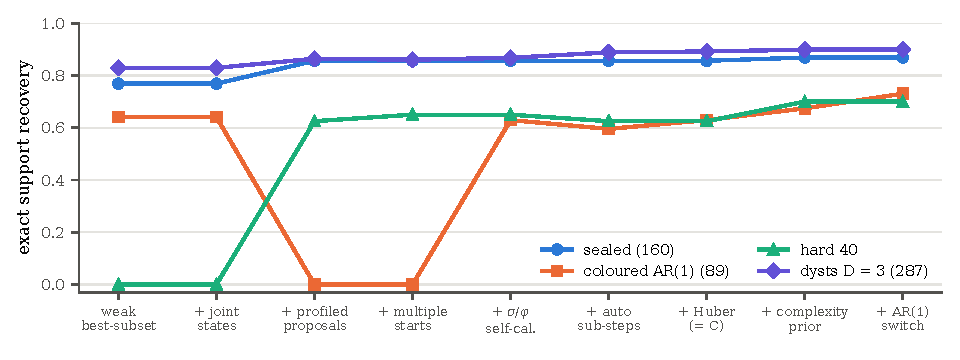
\includegraphics[width=0.92\linewidth]{figures/ablation_ladder.pdf}
\caption{Cumulative ladder from the weak best-subset selector to our method. Up to the last rung the white-noise likelihood is used. Refitting the weak answer jointly (second rung) cannot change its support. The profiled-quadratic proposals give the largest step on white noise, and without self-calibration they overfit every coloured run.}
\label{fig:ladder}
\end{figure}

\paragraph{Subset proposals.} Removing proposals loses 32 exact recoveries and gains none; replacing exhaustive selection with forward stepwise search loses 28 and gains none. On the hard 40, joint refitting of the weak start alone recovers no runs, all starts refitted without proposals recover 19, proposals from the weak start recover 27, and the full method recovers 28. Searching combinations of terms is therefore the principal source of the improvement over refitting existing supports.

\paragraph{Profiling.} A separate prospective ablation builds proposals from $A_{cc}$ and $g_c$, holding the states fixed instead of eliminating their increments. PJSS recovers 490/576 runs versus 480/576 for this variant, with 15 paired wins and 5 losses. On the hard 40 it recovers 28 versus 24; on coloured noise the fixed-state variant has one more recovery. Profiling therefore adds a smaller, setting-dependent gain: it changes how candidates are ranked by accounting for local state adjustment, while both variants retain exhaustive subset proposals and nonlinear joint refits.

\paragraph{Calibration.} Under a white-noise likelihood, proposals overfit every coloured run without noise-scale and penalty calibration; calibration restores recovery in the ladder. Its effect on white noise is negligible. Gaussian loss improves the AR(1) path, motivating the separately confirmed update in \cref{sec:noise}. Other ablations and coefficient errors are reported in \cref{app:ablation-detail}.
